\chapter{Memory Management by the O/S}
\label{chap:memory_management}

Memory management is an essential part of every program. There are different
types of memory; each one has a different memory access speed
\begin{itemize}
  \item registers: the fastest memory space, organized in memory banks. There
  are dedicated registers to store critical information, e.g. instruction
  pointer, or stack pointer.
  
  The amount is limited.
  
  \item physical memory (RAM): the memory where data are physically stored
  during the running of the machine.
  
  This is limited by the amount of RAM installed, e.g. 8GB or 16GB. A 32-bit O/S
  can use maximum 4GB of physical memory. A 64-bit O/S can use maximum 64GB of
  physical memory.
  
  \item file storage: the persistent memory storage like harddisk
    
  \item virtual memory: each application is given a separated virtual memory
  space. This is the memory space that developers directly manipulate at runtime. How
  it is mapped to the locations on the physical memory is controlled by the
  O/S, and as an application developer, we never manipulate physical memory
  directly. A virtual memory address can be in one of 3 states:
  \begin{enumerate}
    \item free : no reference to it and is available for allocation
    \item reserved: is available for use, and cannot be used for any other
    allocation request. However, we cannot store data to this memory until it is
    committed.
    \item committed: the block of memory is assignd to a physical storage (in
    RAM or pagefile (part of harddisk being used as extended RAM)).
  \end{enumerate}
  As memory blocks in the virtual memory will be mapped to physical storage; the
  virtual space can be fragmented if the memory blocks assigned to them from the
  physical storage are not contiguous.
  
  On 32-bit O/S, each process is given maximum 2GB user-mode virtual address
  space. To enable using 3GB or 4GB-mode virtual address space, we need to use
  \verb!/3GB! switch or \verb!/LARGEADDRESSAWARE! linker option.
  \url{http://msdn.microsoft.com/en-us/library/windows/desktop/aa366778(v=vs.85).aspx}

  \begin{enumerate}
    
      \item static data area (SDA): store static and global values 
  
  \item stacks: keep thread-specific and function-related information (e.g.
  local variables, parameters, return values, instruction pointer of the
  calling function, \ldots)
  
  A stack has many stack frame, each stack frame keep the information for one
  functional call.
  
  \item thread local storage (TLS): contain thread-specific information
  (Sect.\ref{sec:TLS}).
  
  \item heaps: keep memory allocated at runtime from the virtual memory
  of the application. Each application can have more than one heap. One heap
  is mapped to the physical memory space by the {\it heap manager}.  
  
  Large objects are often put into the heap; while small objects are put into
  the stack.
  
  \end{enumerate}
  
\end{itemize}

\section{Persistent memory vs. Non-persistent memory}

Persisten memory stores data permanently, regardless with or without power
supply. Examples of persistent memory include harddisk, tapes.

Non-persistent memory stores data only when there is a power supply. 
Examples of non-persistent memory include registers, cache memory (L1, L2 or
L3), RAM. At the lowest level, this is organized by billions of capacitors in
the form of 0s and 1s.

\section{Physical memory vs. Logical memory}

Physical memory is a region of memory, either from RAM or pagefile
(Sect.\ref{sec:pagefile}.  The way memory is stored in the RAM depends
on the RAM architecture.
\begin{itemize}
  \item DRAM: each bit is stored in its own capacitor. A capacitor is an
  electronic device that store a current (mapping to either 0 or 1) for a
  limited of time, thus must be refreshed periodically. 
  \url{http://www.brokenthorn.com/Resources/OSDev17.html}
  
  NOTE: DRAM is not strictly random access, as data is read in bursts, i.e. a
  group of a adjacent memory addresses. However, many SRAM is random-access in
  strict sense.
  
  \item SRAM: Even though the signal doesn't need to periodically refreshed, in
  many SRAM, the data is still {\it volatile} in the sense that it is lost when
  the memory is not powered. The exception is non-volatile SRAM (nvSRAM) which
  are being used in many devices where the preservation of data is critical or
  where batteries are impractical, e.g. networking, aerospace, and medical,
  among many others.
\end{itemize}

In early versions of OS, only single user can use the machine at a time and at
each time, only a single task can run. So, the operating system allows the user
to access the locations on physical memory directly. The program is running in
the so-called {\bf real-address mode}. 8086 CPU only supports real mode. With
20-bit memory address, it supports maximum 1MB of memory, reserves first 640KB
for application and OS, and the 384KB left for BIOS and add-on devices.
% In such situation, compile-time and load-time can be used.
\begin{figure}[hbt]
  \centerline{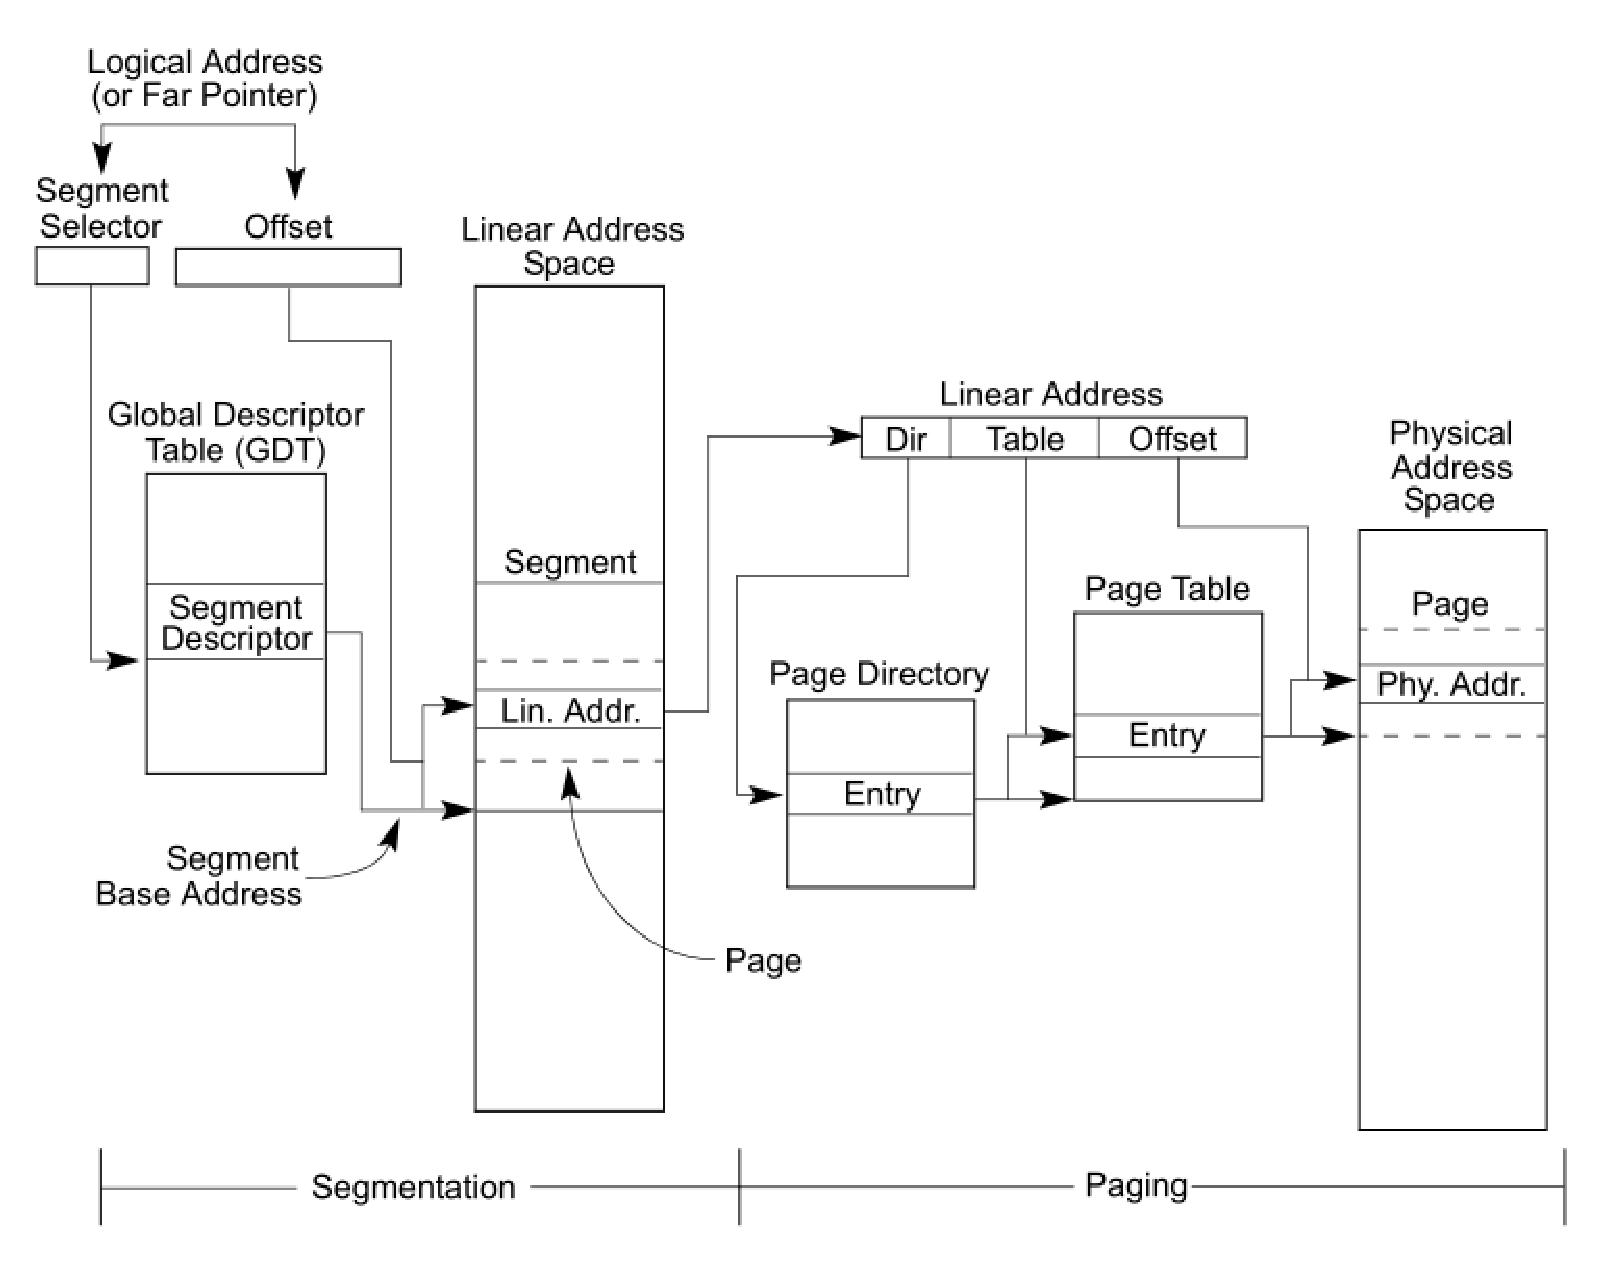
\includegraphics[height=8cm,
    angle=0]{./images/memory_segment.eps}}
\caption{Segmentations}
\label{fig:memory_segment}
\end{figure}

\begin{figure}[hbt]
  \centerline{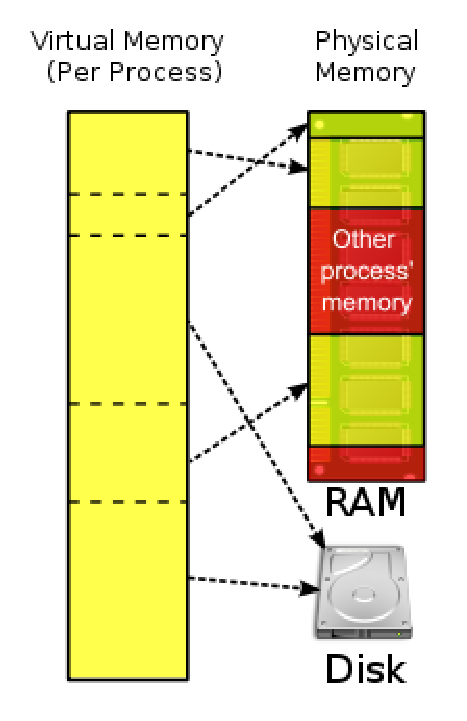
\includegraphics[height=5cm,
    angle=0]{./images/virtual_memory.eps}}
\caption{Virtual memory}
\label{fig:virtual_memory}
\end{figure}

Since 1982, with 80286 CPU, to support multi-tasking, as well as multi-user,
another layer of memory management is added to the kernel of the operating
system. In multi-tasking, the O/S enables the user to switch from one program
to another without exit the current program. As the data of the two programs
are loaded into the memory at the same time, there must be a mechanism to making
sure they are not messing up the data from each other. This is called a {\bf
virtual memory} with a number of modes.

The virtual memory is divided into two parts: user-mode space, and
kernel space, as shown in Fig.~\ref{fig:virtual_address}. They are
normally in the ratio 2G/2G in Windows and 1G/3G in Linux, as shown in
Fig.~\ref{fig:kernel_user}.  The kernel spaces for all processes map
to the same physical kernel space; while the user-mode space from two
different processes never map to the same physical memory location. 
This to ensure the integrity of the O/S, and to protect the O/S from being
attacked by the malicious programs (e.g. virus).

\begin{figure}[hbt]
  \centerline{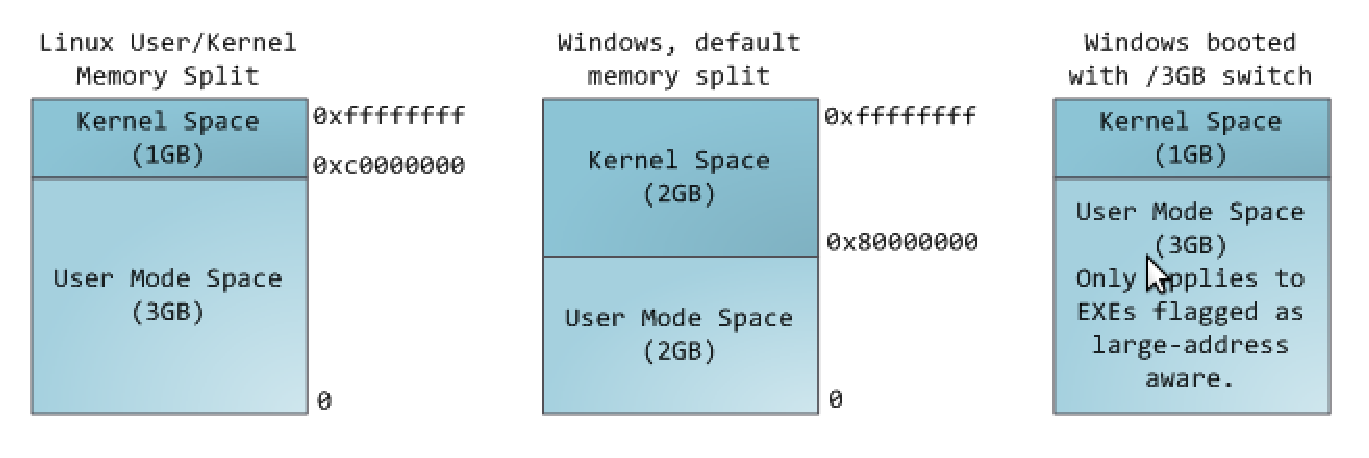
\includegraphics[height=4cm,
    angle=0]{./images/kernel_user_memory.eps}}
\caption{Kernel and User-mode memory space}
\label{fig:kernel_user}
\end{figure}

The {\bf protected mode} was developed to avoid the conflict of memory being
used by one program to another. This virtual memory space are organized into
smaller protected address space called {\it segments}, with code and data are
put into seperates segments (register DS=data segment, and register CS=code
segment). One program cann't access code-segment or data-segment of another
program. A logical address is formed by \verb!segment:offset! pair,
Fig.\ref{fig:memory_segment}. In the basic/protected {\bf flat-model}, only two
segments are created: code segment and data segment being used for all running
programs. In the {\bf multi-segment model}, there are other segments: stack
segment, and more than one data segments.

\begin{enumerate}
  \item in 32-bit addressing: a 16-bit segment registers was introduced that point to the
segment being used by one program, and 32-bit offset selector
\item in 16-bit addressing: a 16-bit segment registers was introduced that point to the
segment being used by one program, and 16-bit offset selector
\end{enumerate} 
The kernel of the O/S will take cares of mapping the logical address to the
physical memory address. 

It's important to know that even though in theory each process has 4GB of
virtual memory, the total memory of all loaded processes, must be less than the
amount of RAM installed + pagefile size (i.e. the amount of hard drive space
being used as RAM). 


\begin{mdframed}
If using 32-bit to address a memory position in the virtual address space, the
maximum linear address space is $2^{32}-1$ (in 32-bit) and $2^{16}-1$ (in
16-bit) which is about 4GB in 32-bit. Since P6 family CPUs, IA-32 architecture
supports $2^{36}-1$=64GB of memory.  
\end{mdframed} 

\section{Pagefile (Windows) vs. Swap space (Linux)}
\label{sec:pagefile}

To allow a program running that uses an amount of memory larger than those
availabel on RAM, Windows O/S  use a fraction of harddisk as
virtual RAM (pagefile). The technique is called {\bf paging} (which can be used with
any segment models).
Paging supports a virtual memory enironment. Here, the processor operates in protected mode; and the
operating system provides virtual management system, e.g. {\bf PAE paging
mechanism}. Example: in 16-bit system, programs run on their own
virtual memory space of 24-bit address line. Then, each program has 16MB virtual
memory space. The OS will manage the mapping this contiguous virtual memory to,
not necessary contiguous, physical main memory and hard drive space, as shown in
Fig.~\ref{fig:virtual_memory}. This make the programming easier as it hide the
fragmentation of data on physical memory.  

In paging, each segment is divided into pages (typically of size 4KByte), which
can be mapped to either physical RAM or harddisk. The operating maintains a
single page-directory and a set of page-tables to keep tracks of pages. A
logical address requires a page-index, and page-offset and map them to physical
address. If the page being access is not in the RAM (as it can be in the
harddisk), a {\it page-fault error} occurs, and the operating system read the
page from harddisk to RAM before continue execution of the program. 




% OS, if all processes are put on the same physical space, how can we
% divide the space to each process. It's not easy as some process is
% large, some is smaller. In addition, one process may access to the
% memory location of another one. To avoid all of these problems, the OS
% create an intermediate layer, by allow each process to have its own
% memory space, known as {\bf virtual memory space}. And the OS will
% manage the loading of codes to virtual memory, as well as mapping it
% to the real physical memory location, as shown in
% Fig. \ref{fig:virtual_address}, when it issues the instruction to CPU.

\begin{figure}[hbt]
  \centerline{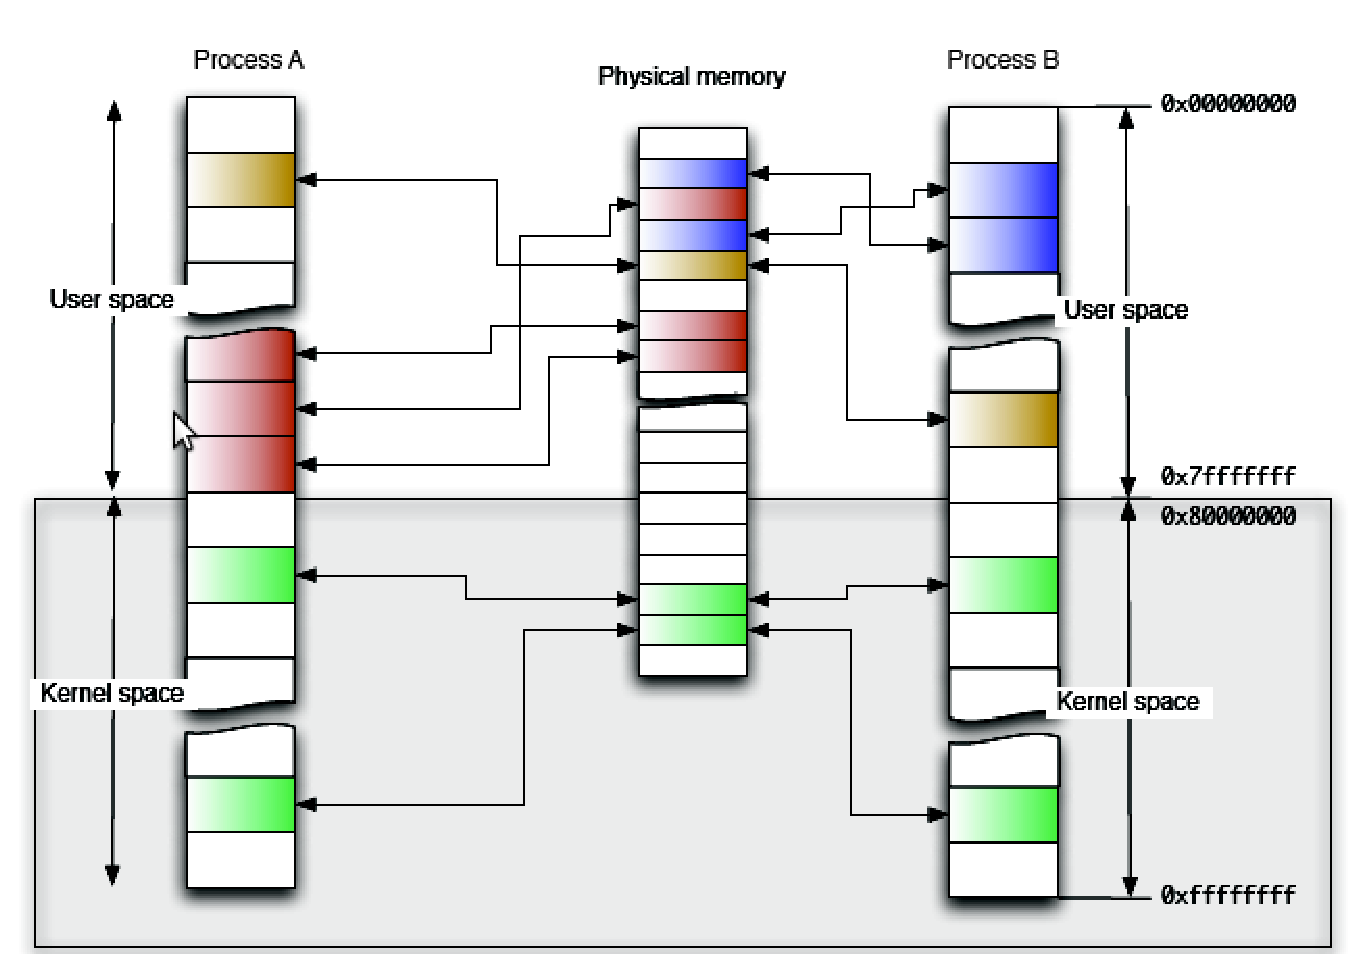
\includegraphics[height=5cm,
    angle=0]{./images/virtual_address.eps}}
\caption{Virtual address}
\label{fig:virtual_address}
\end{figure}

Using virtual memory design, almost all implementation divide the
virtual memory space into blocks of contiguous virtual memory space,
known as {\bf pages}. Pages are homogeneous blocks of 4KB, in most
32-bit systems. Systems with large virtual memory space or large RAM,
generally use larger page size.  They are mapped to physical address
by {\bf page tables} which are maintained by the OS.  With 4GB of
memory, we need 1 Mega (1024x1024) 4KB pages. The CPU use a two-level
structure to map a page to a physical memory location. Consider it as
a 1024x1024 matrix, with the first dimension is Page Directory and the
second dimension is known as the Page
Table\footnote{\url{http://www.intellectualheaven.com/Articles/WinMM.pdf}}.
So, we have 1024 Page Directory, each Page Directory has 1024 Page
Tables, each Page Table has 1024 entries, each of which points to the
initial address of a 4KB page in physical memory, as shown in
Fig.~\ref{fig:paging}.

\begin{figure}[hbt]
  \centerline{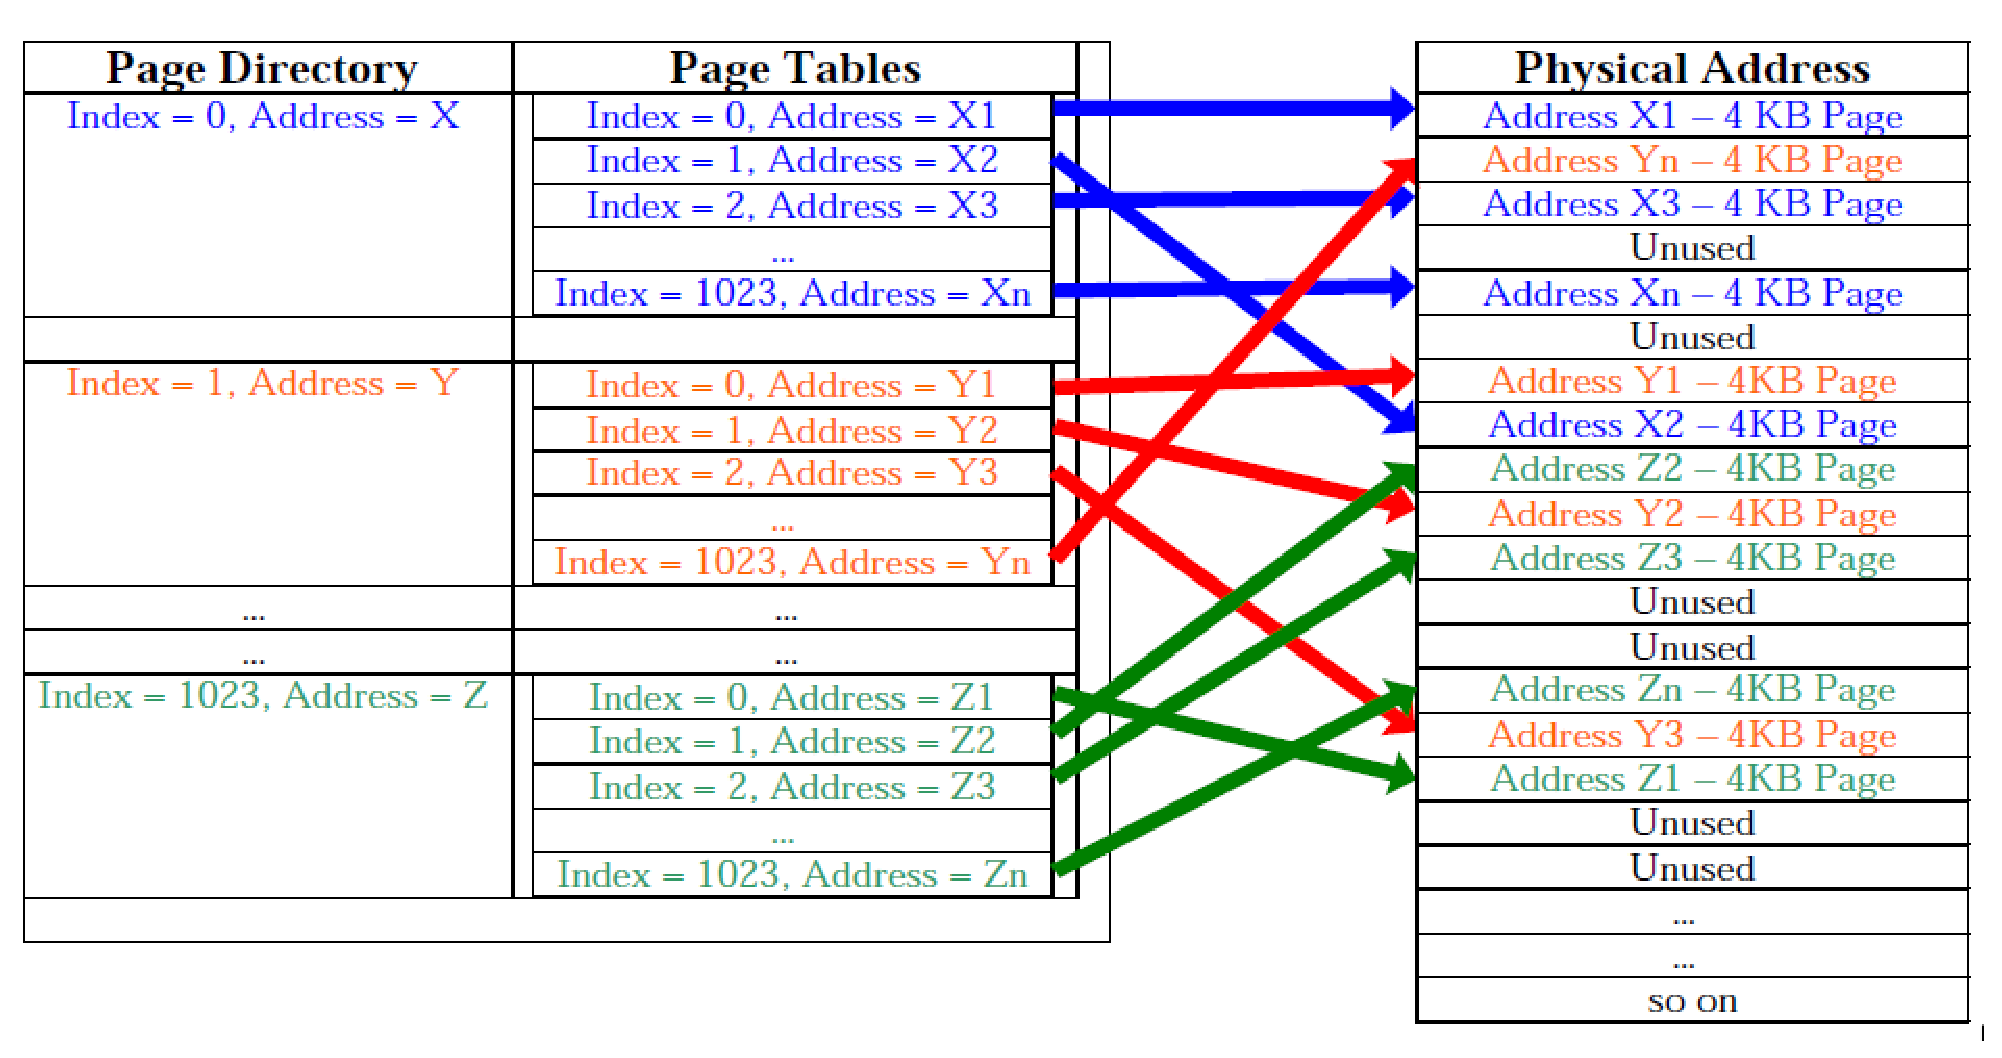
\includegraphics[height=5cm,
    angle=0]{./images/paging.eps}}
\caption{Paging}
\label{fig:paging}
\end{figure}

The total amount of the memory to store Page Directory + Page Table is
4MB = 1024x1024x4. In Windows, each process has its own PD and PT;
thus at least it use 4MB of RAM when it is loaded. The starting
address where the whole PD and PT is stored in RAM is known as
{\bf Page Directory Base} address which is stored in the special CPU
register CR3 (on x86). So, when context switching occur, i.e. CPU
serve a different process, the value of CR3 is changed to the value of
the address of the PDB of the new process, as shown in
Fig.~\ref{fig:paging_register}.
\begin{figure}[hbt]
  \centerline{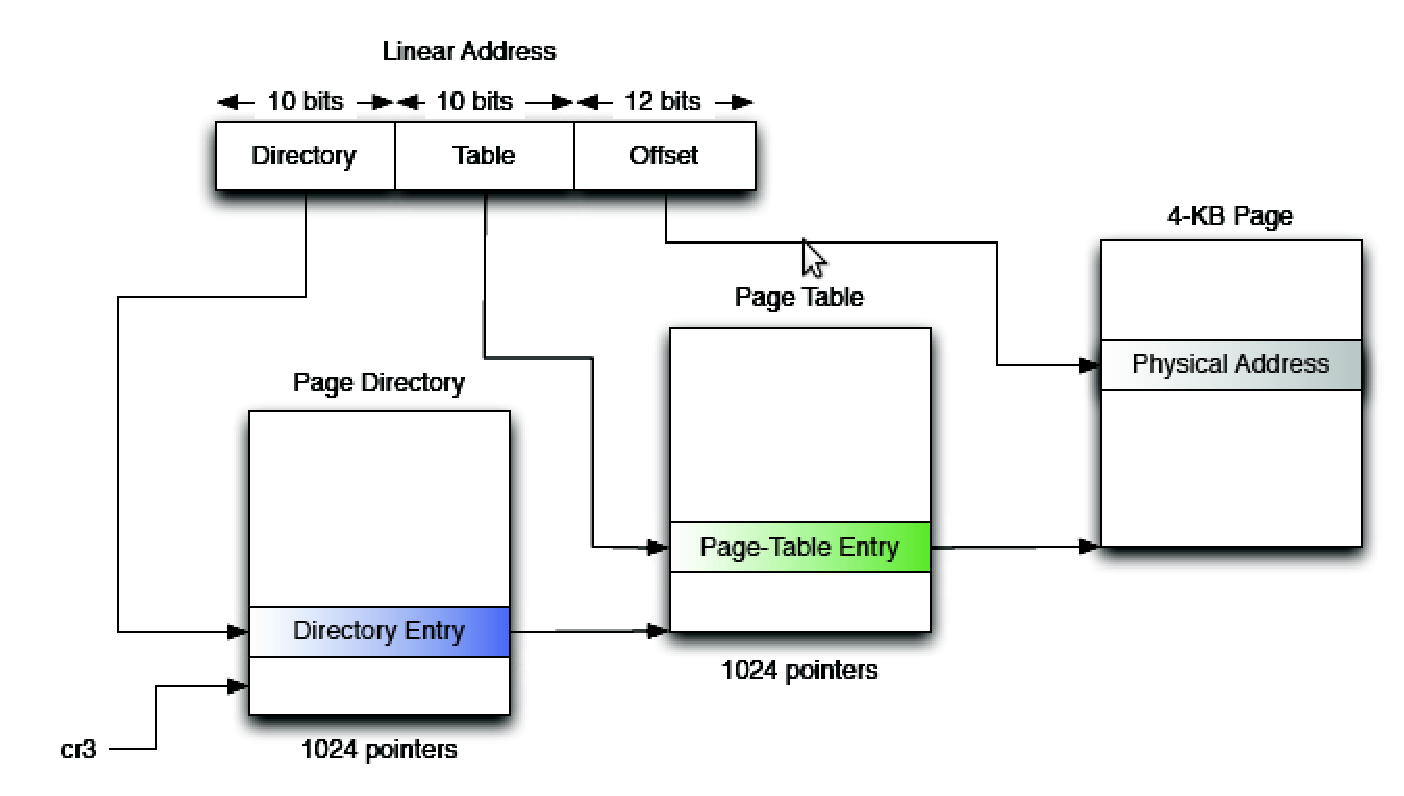
\includegraphics[height=5cm,
    angle=0]{./images/paging_register.eps}}
\caption{Paging and register to address Page Directory, Page Table}
\label{fig:paging_register}
\end{figure}
CR3 is a 32-bit register with the highest 10 bits keep the index of
Page Directory Entry (PDE), the next 10bits keep the index of the Page
Table Entry (PTE), and the last 12 bits to address the individual
bytes in the page (which can address any byte within the 4KB
limit). To avoid user change Page table information, the total 4MB
resides in the kernel logical space, with logical address 0xC000000000
to store the Page Tables and address 0xC0300000 to store page
directory. \textcolor{red}{For 64-bit system, read
  Sec.~\ref{sec:64-bit-systems}.}


{\bf NOTE}: Some virtual pages do not map to any actual physical
memory address, because not all virtual pages are necessarily being
used at any given time; these unused virtual pages are called
invalid. If a program ever tries to access an invalid page, the CPU
traps to the operating system, causing a Segmentation Fault or Access
Violation.

Other systems, rather than use pages, implement a different technique,
known as {\bf segmentation} of variable-length segments. Some systems
combine the two designs, i.e. virtual space is divided into segments,
each segment is divided into pages.

When a program access the unexpected memory, the error
{\it segmentation fault} or {\it general protection fault} occurs,
e.g. de-references a NULL pointer.  However, when running multiple
programs, the memory required is often exceed the RAM installed,
Windows developed create a so-called {\bf pagefile} that use an amount
of physical hard drive spaces to stored the data as RAM. Of course,
accessing data in page memory is slower than in RAM. So, when there is
not enough page in RAM, it save the data to pagefile. We call this
{\bf page eviction}. When these pages are accessed again, the OS
restore theme back to the physical RAM, possibly evicting other
inactive pages to the pagefile. If the process continues to access
pages swap to the disk, then the system will spend most of its time
moving data around from RAM to disk; this will slow down the
performance and is called {\bf thrashing}, i.e. the system does lots
of things but make no useful progress. 


In Linux, instead of using pagfile, it reserved a separate partition,
known as {\bf swap space}, which is normally about 2x of RAM
installed.

References:
\begin{enumerate}
\item
  \url{http://www.cs.miami.edu/~burt/learning/Csc521.071/notes/tovm.html}
\item
  \url{http://duartes.org/gustavo/blog/post/anatomy-of-a-program-in-memory}
\item \url{http://duartes.org/gustavo/blog/post/cpu-rings-privilege-and-protection}
\end{enumerate}

% \section{CPU interact with data in memory (registers, cache, RAM, harddisk)}
% 
% The CPU is the central processing unit that can performs different kinds of
% operations, each one needs to use data to perform its tasks. The data can
% be in one of the different memory spaces (registers, cache, RAM or harddisk). 



\section{Thread Local Storage (TLS)}
\label{sec:TLS}

As threads in the same process share the same memory space, it is sometimes
undesirable. Sometimes it is desirable that two threads referring to the same
static or global variable are actually referring to different memory locations,
thereby making the variable thread-local.
\footnote{\url{http://en.wikipedia.org/wiki/Thread-local_storage}}

A TLS table is 64 slots of 32-bit values, which holds pointers to dynamically
allocated memory that belongs to the thread.


\subsection{C++}

\subsection{C\#}

In C\#, static fields can be marked as thread-local with \verb![ThreadStatic]!
attribute
\begin{verbatim}
class FooBar {
   [ThreadStatic] static int foo;
}
\end{verbatim}

Since .NET 4.0, it has
\begin{verbatim}
 private static System.Threading.ThreadLocal<int> foo;
\end{verbatim}
\url{http://msdn.microsoft.com/en-us/library/dd642243.aspx}


\section{Memory in Win32}
\label{sec:memory-Win32}

Win32 functions allocate memory and put them on {\bf native heap}. There is no
memory manager for this heap; so it is the task of the programmer to free the
memory once it is no longer being used.

Fig.\ref{fig:memory-management-Win32} provides details of how memory objects are
allocated. Depending on the location of the data, Win32 provides 3 groups of
APIs: memory-mapped file functions, heap memory functions, and virtual memory
functions.

\begin{figure}[hbt]
  \centerline{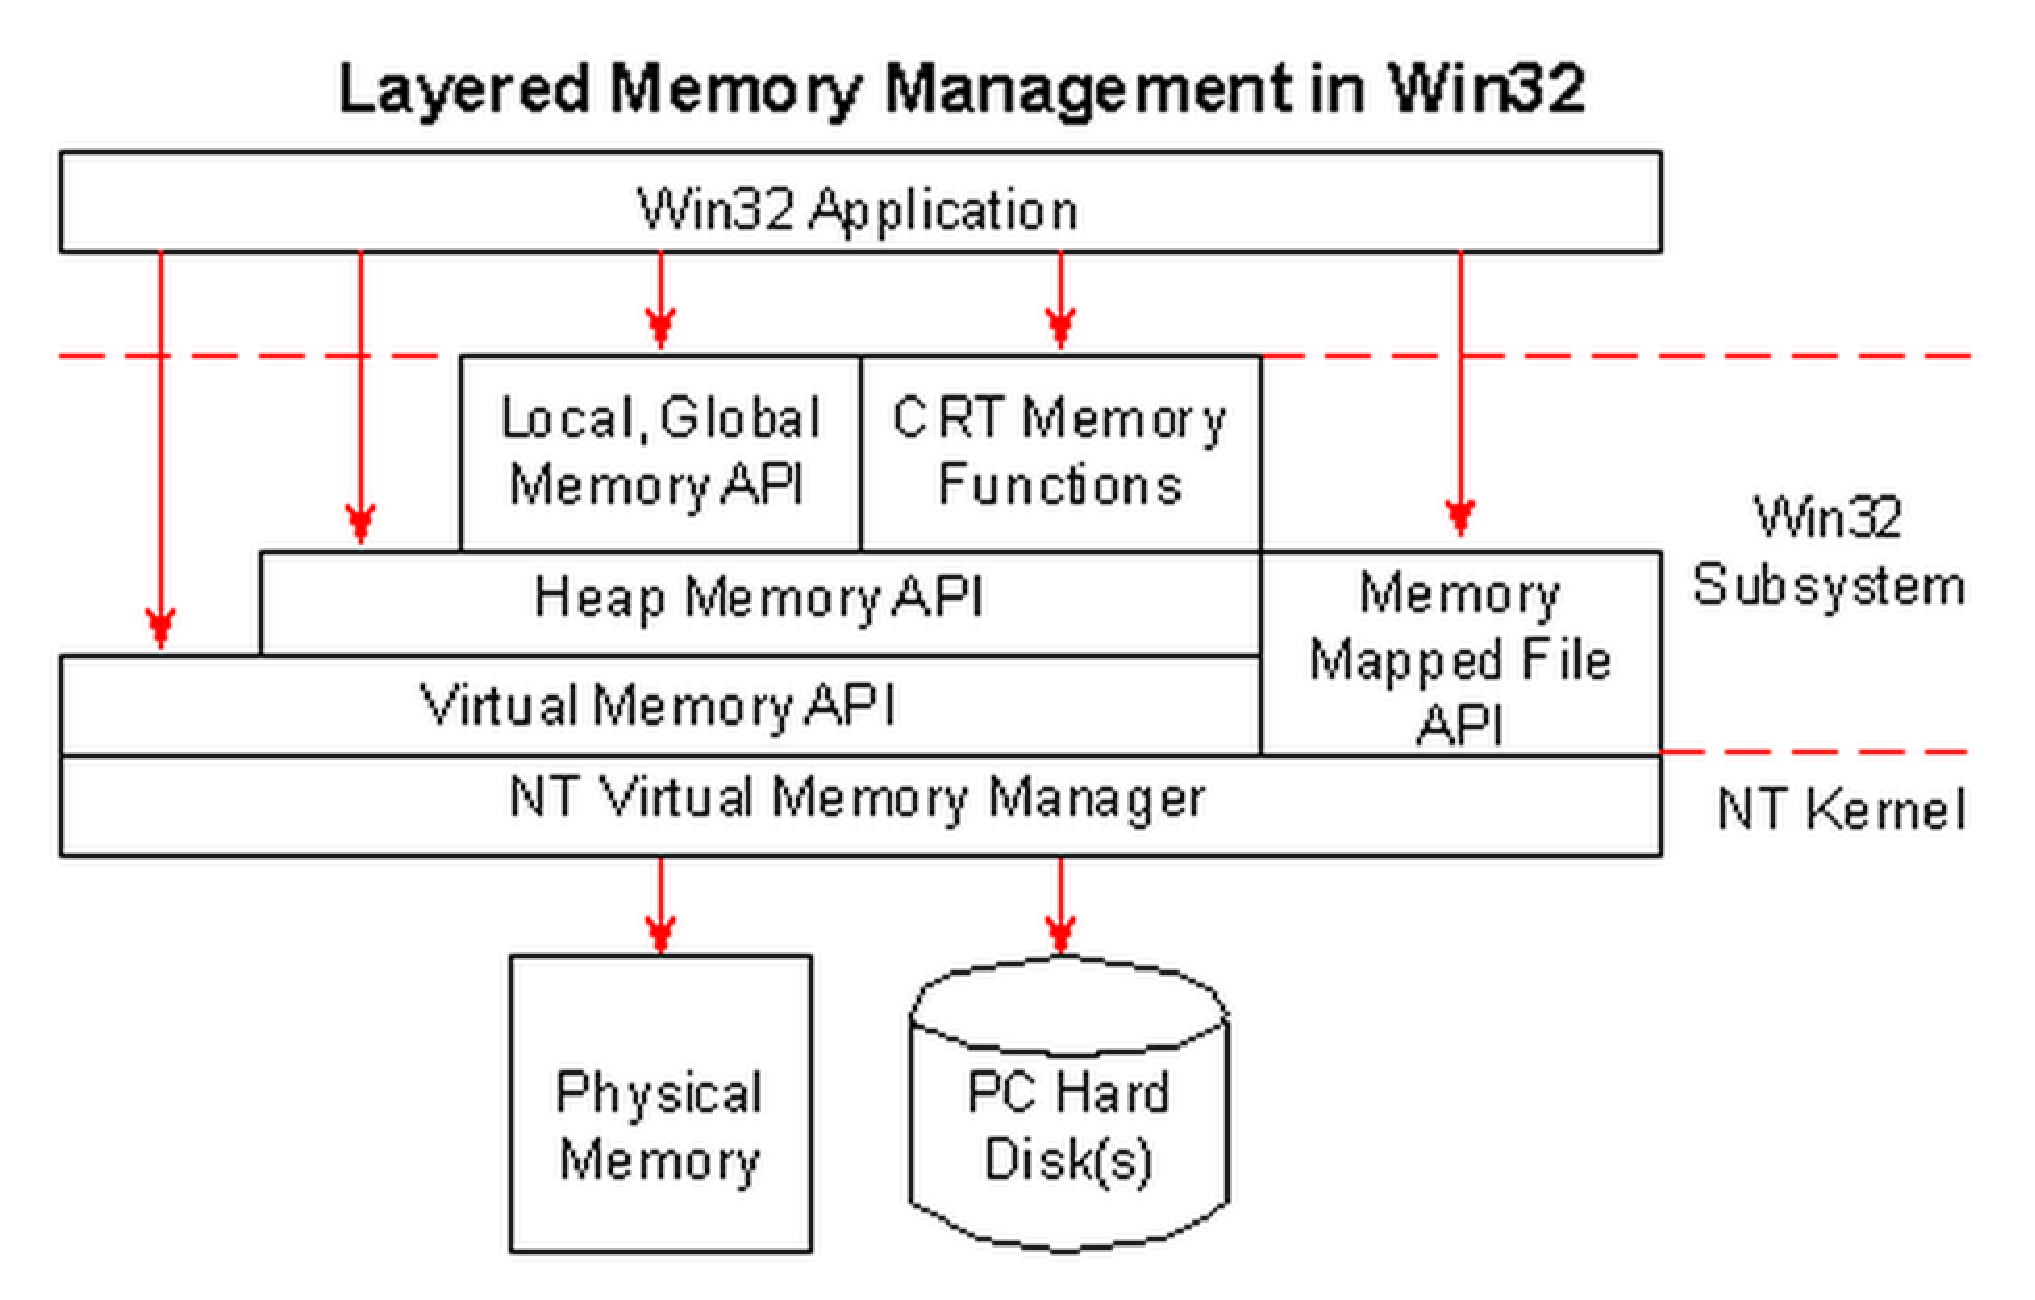
\includegraphics[height=5cm,
    angle=0]{./images/memory-management-win32.eps}}
  \caption{Layers of Memory Management in Win32}
\label{fig:memory-management-Win32}
\end{figure}

\url{http://msdn.microsoft.com/en-us/library/ms810603.aspx}

Generally spoken, Windows offers applications three ways of allocating memory:
{\bf virtual memory}, {\bf shared memory} and {\bf heaps}. The first one is the
primary means by which SQL Server allocates memory when that's needed. The
virtual memory functionality in the Windows OS can be summarized by explaining
the some key functions in the Win32 API to work with this mechanism. Check the
APIs from Platform SDK of Windows XP and Windows Server 2003.

\subsection{Virtual Memory}
\label{sec:virtual-mem-alloc-Win32}

\begin{enumerate}
  \item VirtualAlloc/VirtualFree
  
  \item VirtualLock and VirtualUnlock: to lock the virtual memory in the
  physical memory
  
  \item VirtualProtect: change the protection attributes of a virtual memory
  page; examples of these attributes are 
  \begin{verbatim}
  PAGE_EXECUTE, 
  PAGE_EXECUTE_READ,
  PAGE_EXECUTE_READ_WRITE
  \end{verbatim}
  , etc including support for copy-on-write mechanisms and so on
  
  \item VirtualQuery: obtain information about the virtual memory on the system 
\end{enumerate}

\subsection{Heap memory}

A heap is controlled by a thing called a heap manager and consists of a region
in memory divided in pages of reserved space. The heap manager can be called to
get a piece of memory to work with. Typically heaps are used when objects or
structures with similar sized need to be allocated in memory. An example of the
usage of a heap is the {\bf new} operator in C++ or the {\bf malloc} function in
C.
\begin{enumerate}
  \item HeapCreate and HeapDestroy : create/destroy the so-called private heap
  \item HeapAlloc: like C's malloc()
  \item HeapFree: like C's free()
\end{enumerate}

\subsection{Shared memory}

The idea of shared memory is to allocate a memory region and to allow shared
access to it for multiple processes, so it can be used for inter process data
exchange. 

SQL Server uses shared memory as a fast way to communicate with client
applications {\it on the same machine}, bypassing protocols such as TCP/IP (and
therefore the whole network OSI stack) or named pipes, through the Net-Library
related functionality  

\begin{enumerate}
  \item CreateFileMapping: create a {\it section object} to be used with either
  shared memory or a memory-mapped file
  
  \item MapViewOfFile: creates a mapped view for a file in the physical memory
  
  \item FlushViewOfFile: write the modified pages in the mapped view to disk
\end{enumerate}

\subsection{File mapping}
\label{sec:FileMapping-Win32}

File mapping is the association of a file's contents with a portion of the
virtual address space of a process. The system creates a file mapping object
(also known as a section object) to maintain this association. A file view is
the portion of virtual address space that a process uses to access the file's
contents. File mapping allows the process to use both random input and output
(I/O) and sequential I/O. It also allows the process to work efficiently with a
large data file, such as a database, without having to map the whole file into
memory. Multiple processes can also use memory-mapped files to share data.    

\begin{Verbatim}
//C++
LPVOID WINAPI MapViewOfFile(
  _In_  HANDLE hFileMappingObject,
  _In_  DWORD dwDesiredAccess,
  _In_  DWORD dwFileOffsetHigh,
  _In_  DWORD dwFileOffsetLow,
  _In_  SIZE_T dwNumberOfBytesToMap
);

UnmapViewOfFile
\end{Verbatim}
To specify a suggested base address for the view, use the MapViewOfFileEx
function. However, this practice is not recommended.

The file on disk can be any file that you want to map into memory, or it can be
   the system page file. A process can create multiple views for a file mapping
   object. When multiple processes use the same file mapping object to create
   views for a local file, the data is coherent. That is, the views contain
   identical copies of the file on disk, Fig.\ref{fig:FileMapping}. The file
   cannot reside on a remote computer if you want to share memory between multiple processes.  
   
\begin{figure}[hbt]
  \centerline{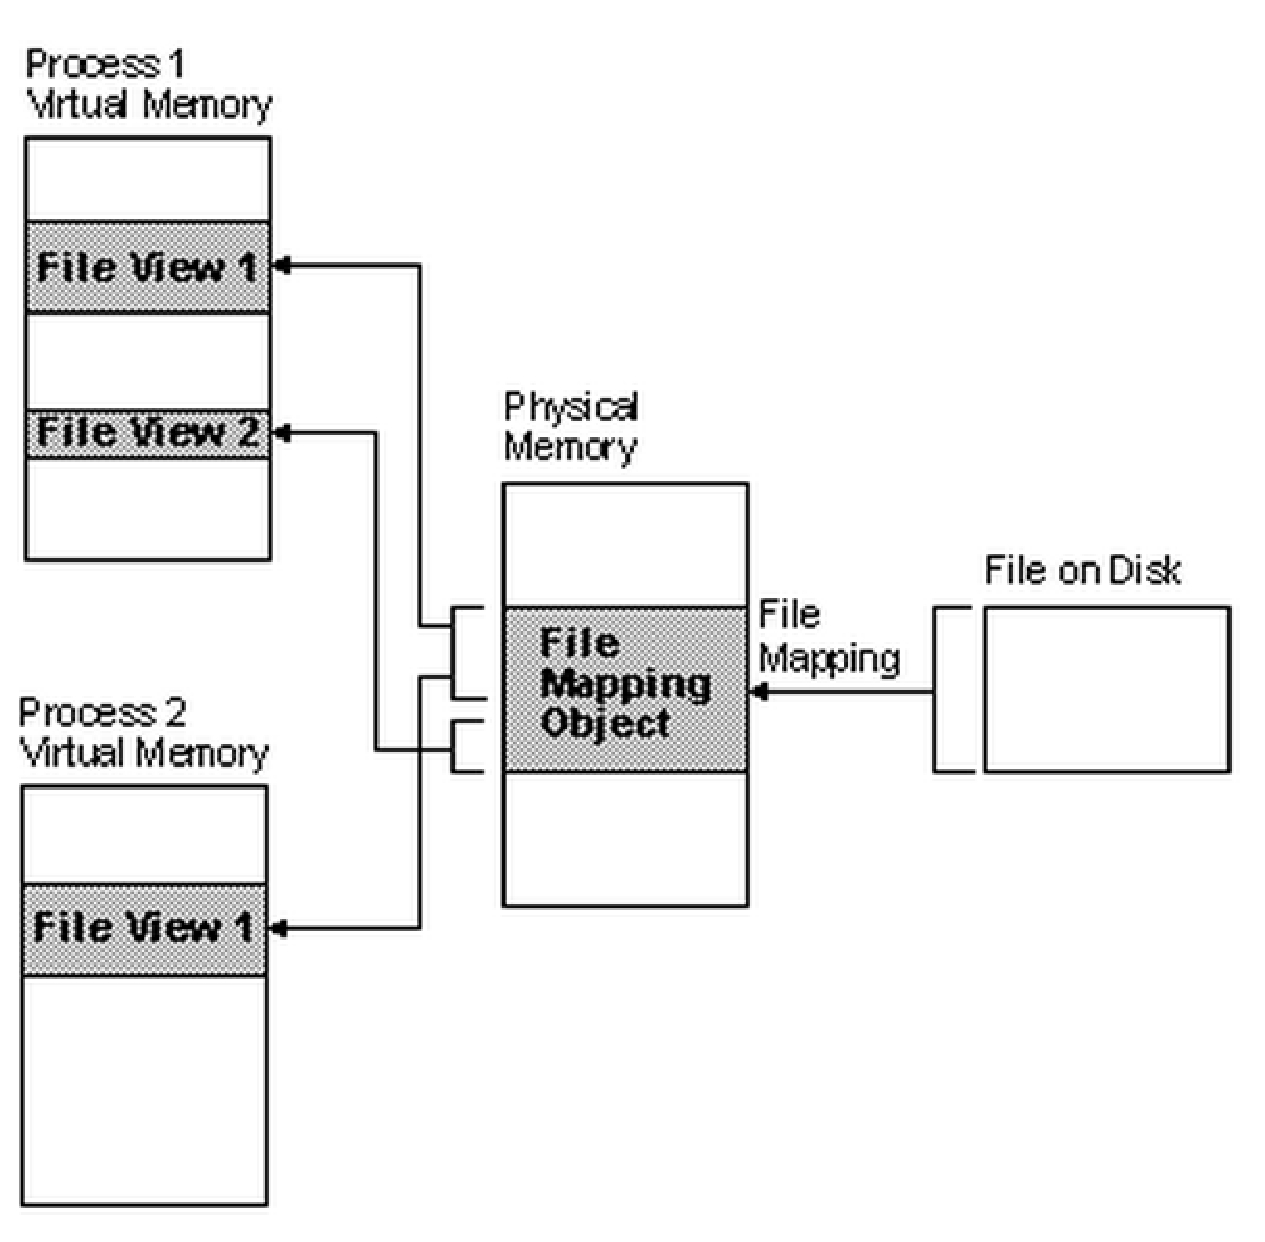
\includegraphics[height=5cm,
    angle=0]{./images/FileMapping.eps}}
  \caption{File Mapping}
\label{fig:FileMapping}
\end{figure}

The equivalent call in Unix is  mmap(2) Unix system call.   

\url{http://msdn.microsoft.com/en-us/library/windows/desktop/aa366556(v=vs.85).aspx}
